\documentclass{../../slides-style}

\slidetitleext{Логическое программирование}{12.05.2023}{Prolog}

\begin{document}
    
    \frame{\titlepage}

    \section{Введение}
    
    \begin{frame}
        \frametitle{Историческая справка}

        \begin{tabular}{m{1cm}m{10cm}}
             \textbf{1951} & Альфред Хорн выделил и изучил дизъюнкты специального вида, который назвали в честь него (\textit{Америка})\\[5mm]
             \textbf{1970-1975} &
             Роберт Ковальски показал, что логическое доказательство может быть вычислено\footnote{\href{http://www.doc.ic.ac.uk/~rak/papers/IFIP\%2074.pdf}{\footnotesize{Predicate Logic as a Programming Language, University of Edinburgh, 1973}}} (\textit{Великобритания}) \\[5mm]
             \textbf{1972} & Ален Колмероэ и Филипп Руссель разработали язык Пролог (\textit{Франция}) \\[5mm]
             \textbf{1982-1992} & Один из основных языков разработки базы знаний в национальном проекте ``Пятое поколение компьютеров'' \newline (\textit{Япония})
        \end{tabular}
    \end{frame}

    \begin{frame}
        \frametitle{Programmation en logique}
        \begin{itemize}
            \item Prolog --- аббревиатура от ``\textit{programmation en logique}''
            \vspace{2mm}
            \item \textbf{Язык} и \textbf{система} логического программирования
            \begin{itemize}
                \item Хорновские выражения (предикаты первого порядка)
                \item Метод резолюции
                \item Унификация
                \item Поиск с ограничениями в древовидной структуре
                \begin{itemize}
                    \item Возможно, бесконечной
                \end{itemize}
            \end{itemize}
            \vspace{2mm}
            \item Язык декларативного программирования
            \vspace{2mm}
            \item Cуществует множество диалектов
            \begin{itemize}
                \item Datalog
                \item $\alpha$Prolog
                \item $\lambda$Prolog
                \item $\ldots$
            \end{itemize}
        \end{itemize}
    \end{frame}

        \begin{frame}
        \frametitle{В индустрии}
        \begin{itemize}
            \item IBM Watson 
            \begin{itemize}
                \item Система синтеза ответов для вопросов на естественном языке
                \item Сопоставление с образом на деревьях разбора естественных языков
            \end{itemize}
            \vspace{2mm}
            \item GeneXus 
            \begin{itemize}
                \item Визуальный кроссплатформенный инструмент разработки
                \item Преобразование визуальной программы в код для конкретной платформы
            \end{itemize}
            \vspace{2mm}
            \item TerminusDB
            \begin{itemize}
                \item Графовая база данных
                \item Похожа на git
                \item Реализована на Prolog
            \end{itemize}
        \end{itemize}
    \end{frame}

    \begin{frame}
        \frametitle{Где попробовать}
        \begin{itemize}
            \item SWI-Prolog
            \begin{itemize}
                \item Свободная реализация интерпретатора Пролога
                \item Есть web-версия
                \begin{itemize}
                    \item  \href{https://swish.swi-prolog.org/}{https://swish.swi-prolog.org/}
                \end{itemize}
            \end{itemize}
            \vspace{2mm}
            \item Есть реализация интерпретатора под .NET
            \begin{itemize}
                \item \href{https://github.com/Slesa/Prolog.NET}{https://github.com/Slesa/Prolog.NET}
            \end{itemize}
            \vspace{2mm}
            \item Минималистичная реализация на OCaml
            \begin{itemize}
                \item \href{https://github.com/dboulytchev/microProlog}{https://github.com/dboulytchev/microProlog}
            \end{itemize}
             \vspace{2mm}
            \item ...
        \end{itemize}
    \end{frame}

    \begin{frame}
        \frametitle{Начнем с основ}
        \begin{itemize}
            \item Программа (база знаний) представляет из себя набор фактов и правил вывода
            \vspace{2mm}
             \item Факты и правила можно рассматривать как отношения с математической точки зрения
             \begin{itemize}
                 \item На первый взгляд это функции, возвращающие \mintinline{prolog}{bool}
             \end{itemize}
            \vspace{2mm}
            \item Для старта вычисления необходим запрос к базе знаний
            \vspace{2mm}
            \item Результатом являются уточнения запроса, выводимые из базы знаний 
        \end{itemize}
    \end{frame}

\section{Примеры}

    \begin{frame}[fragile]
        \frametitle{Простой пример\footnote{\href{https://swish.swi-prolog.org/example/kb.pl}{https://swish.swi-prolog.org/example/kb.pl}}}
        \begin{columns}
            \column{0.5\textwidth}
            \begin{minted}{prolog}
loves(vincent, mia).
loves(marcellus, mia).
loves(pumpkin, honey_bunny).
loves(honey_bunny, pumpkin).

jealous(X, Y) :-
    loves(X, Z),
    loves(Y, Z).
            \end{minted}
            \column{0.5\textwidth}
            \pause
            \vspace{2mm}
            \begin{minted}{prolog}
?- loves(vincent, mia) -> true
            \end{minted}
            \pause
            \vspace{2mm}
            \begin{minted}{prolog}
?- loves(vincent, pumpkin) -> false
            \end{minted}
            \pause
            \vspace{2mm}
            \begin{minted}{prolog}
?- loves(X, mia) ->
      X = vincent;
      X = marcellus
            \end{minted}
            \pause
            \vspace{2mm}
            \begin{minted}{prolog}
?- jealous(X, Y) ->
      X = Y, Y = vincent;
      X = vincent, Y = marcellus;
      X = marcellus, Y = vincent;
      X = Y, Y = marcellus;
      X = Y, Y = pumpkin;
      X = Y, Y = honey_bunny 
            \end{minted}
        \end{columns}
    \end{frame}

    \begin{frame}[fragile]
        \frametitle{Ещё простой пример}
        \begin{columns}
            \column{0.5\textwidth}
            \begin{minted}{prolog}
append([], X, X).
append([X|Xs], Y, [X|Zs]) :-
  append(Xs, Y, Zs).
            \end{minted}
            \column{0.5\textwidth}
            \pause
            \vspace{2mm}
            \begin{minted}{prolog}
?- append([a], [b,c], [a,b,c]) -> true
            \end{minted}
            \pause
            \vspace{2mm}
            \begin{minted}{prolog}
?- append([a], [b,c], X) -> 
      X = [a,b,c]
            \end{minted}
            \pause
            \vspace{2mm}
            \begin{minted}{prolog}
?- append(X, [c], [a,b,c]) ->
      X = [a,b]
            \end{minted}
            \pause
            \vspace{2mm}
            \begin{minted}{prolog}
?- append(X, Y, [a,b,c]) ->
      X = [], Y = [a,b,c];
      X = [a], Y = [b,c];
      X = [a,b], Y = [c];
      X = [a,b,c], Y = [];
            \end{minted}
        \end{columns}
    \end{frame}

\section{Как устроен Prolog}

    \begin{frame}
        \frametitle{Как это работает} 
        \begin{itemize}
            \item Построение вывода от запроса к фактам 
            \begin{itemize}
                \item Метод резолюций
                \item Перебор возможных путей поиском в глубину с возвратами
            \end{itemize}
            \vspace{2mm}
            \item Унификация
            \begin{itemize}
                \item Уточнение переменных
                \item Проверка, что запрос вложен в факт или в голову правила вывода
            \end{itemize}
        \end{itemize}
    \end{frame}

    \begin{frame}[fragile]
        \frametitle{Дерево поиска}
        \begin{minted}{prolog}
loves(vincent, mia).
loves(marcellus, mia).
loves(pumpkin, honey_bunny).
loves(honey_bunny, pumpkin).
jealous(X, Y) :- loves(X, Z), loves(Y, Z).

?- jealous(X, Y).
        \end{minted}
    \vspace{-15mm}
    \includegraphics[scale=0.57]{prolog-tree.eps}
    \end{frame}

    \begin{frame}
        \frametitle{Дерево поиска}
    \includegraphics[scale=0.57]{prolog-tree-neg.eps}
    \end{frame}

    \begin{frame}[fragile]
        \frametitle{Унификация: определения}
    \begin{itemize}
        \item Термы $\mathcal{T} = \mathcal{V} \mid \mathcal{C} (\mathcal{T}, \, \ldots, \, \mathcal{T})$
        \begin{itemize}
            \item Функциональные символы (конструкторы) и переменные
        \end{itemize}
        \pause
        \vspace{2mm}
        \item Подстановка $\Sigma : \mathcal{V} \rightarrow \mathcal{T}$
        \begin{itemize}
            \item Отображение из имен переменных в термы  
        \end{itemize}
        \pause
        \vspace{2mm}
        \item Применение подстановки $t \, \Sigma$
        \begin{itemize}
            \item Замена в терме $t$ переменных на термы в соответствии с подстановкой $\Sigma$
            \item 
                \mintinline{prolog}{node(X, Y)}
                $\{$
                    \mintinline{prolog}{X} $\leftarrow$ \mintinline{prolog}{node(leaf, Z)}
                $\} = $ \mintinline{prolog}{node(node(leaf, Z), Y)}
        \end{itemize}
        \pause
        \vspace{2mm}
        \item Отношение частичного порядка над подстановками
        \begin{itemize}
            \item $\Sigma_1 < \Sigma_2$, если $\exists\; \Sigma\; \forall\; t \in \mathcal{T} \quad t\,\Sigma_1\Sigma = t\,\Sigma_2$
            \item Подстановка меньше, если содержит меньше информации
        \end{itemize}
    \end{itemize}
    \end{frame}

        \begin{frame}[fragile]
        \frametitle{Унификация}
    \begin{itemize}
        \item Унификатор для термов $t_1$ и $t_2$
         \begin{itemize}
            \item Подстановка $\Sigma$ такая, что $t_1\,\Sigma = t_2\,\Sigma$
            \item Унификатора может не быть
            \item Унификаторов может быть много
        \end{itemize}
        \pause
        \vspace{2mm}
        \item Унификация $unify : \mathcal{T} \rightarrow \mathcal{T} \rightarrow \Sigma\, option$
        \begin{itemize}
            \item Построение наименьшего унификатора для двух термов
            \item На самом деле, $unify : \Sigma\; option \rightarrow \mathcal{T} \rightarrow \mathcal{T}  \rightarrow \Sigma \;option$
            \item В худшем случае экспоненциальна
            \item Сопоставление с образцом --- частный случай унификации
        \end{itemize}
    \end{itemize}
    \end{frame}

    \begin{frame}
        \frametitle{Унификация: пример 1}
    \begin{tabular}{m{25mm}cm{25mm}cm{25mm}}
    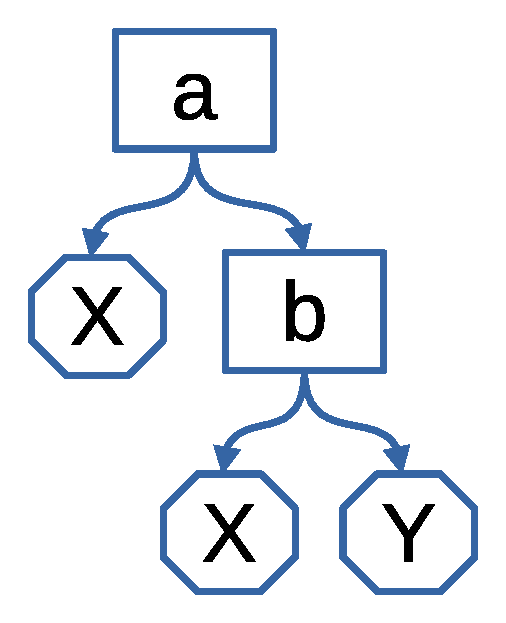
\includegraphics[scale=0.4]{term1.eps} &
    \textbf{\Huge $\equiv$} &
    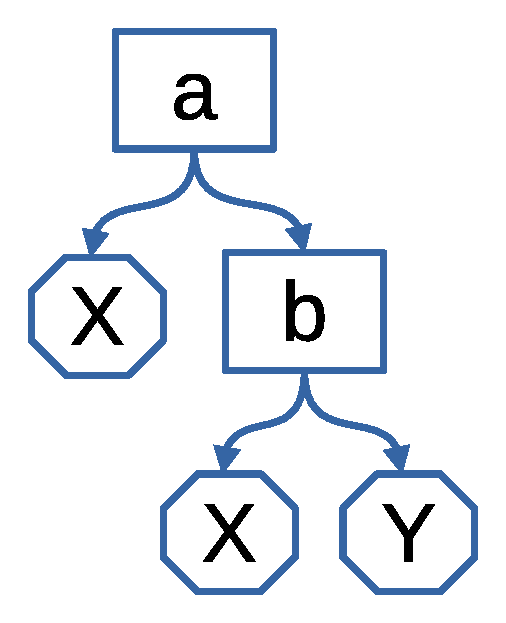
\includegraphics[scale=0.4]{term1.eps} &
    \textbf{\Huge $\Rightarrow$} &
    \pause     
    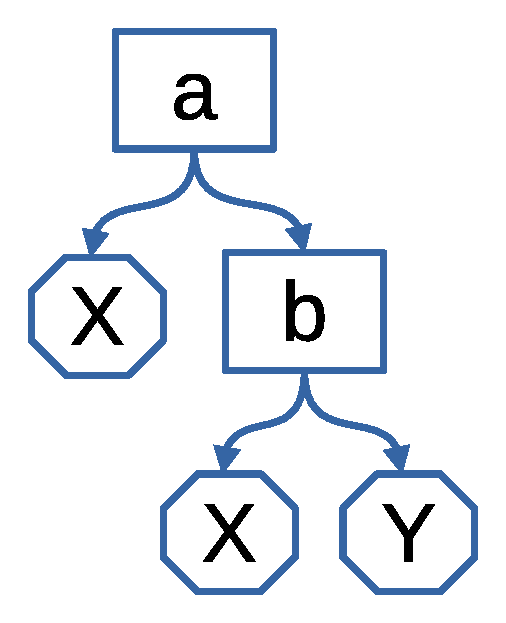
\includegraphics[scale=0.4]{term1.eps}
    \end{tabular}
    \end{frame}

    \begin{frame}
        \frametitle{Унификация: пример 2}
    \begin{tabular}{m{25mm}cm{25mm}cm{25mm}}
    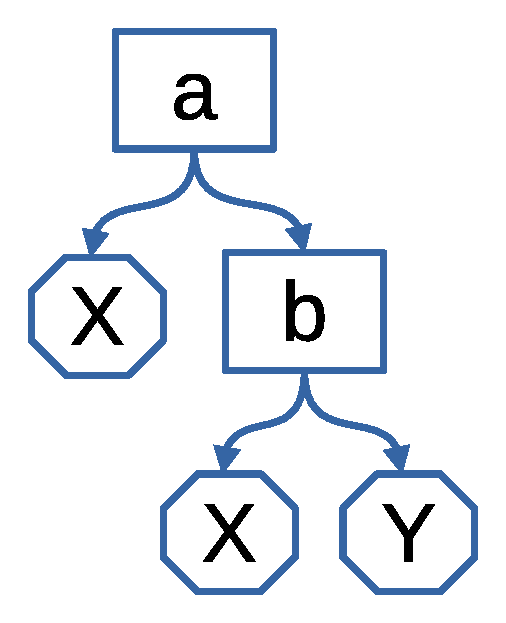
\includegraphics[scale=0.4]{term1.eps} &
    \textbf{\Huge $\equiv$} &
    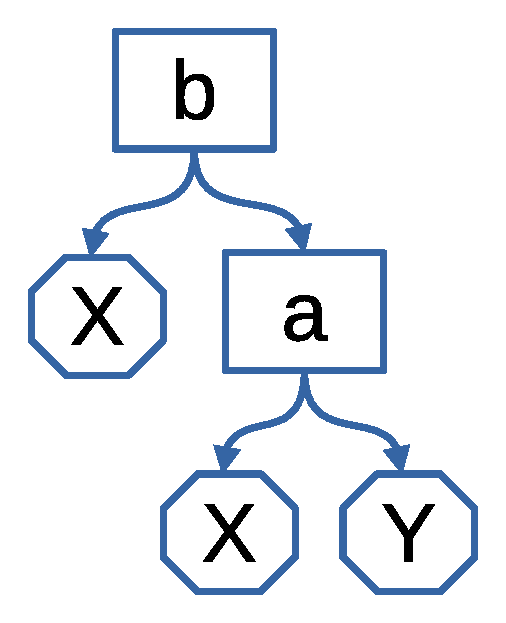
\includegraphics[scale=0.4]{term2.eps} &
    \textbf{\Huge $\Rightarrow$} &
    \pause \centering
    \vspace{-2mm}
    \textbf{\Huge fail}
    \end{tabular}
    \end{frame}

    \begin{frame}
        \frametitle{Унификация: пример 3}
    \begin{tabular}{m{25mm}cm{25mm}cm{25mm}}
    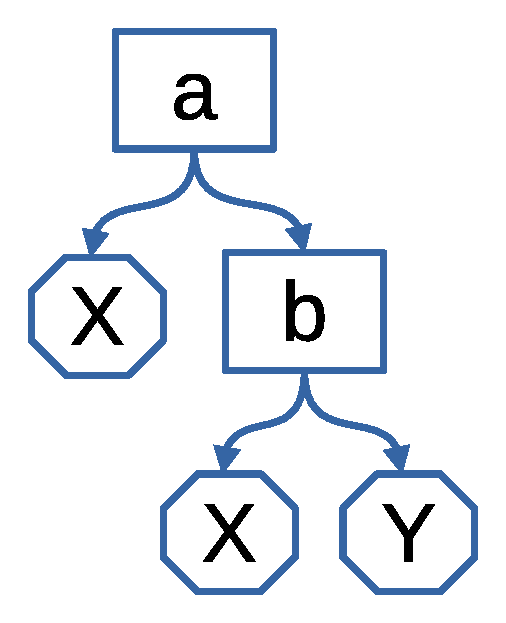
\includegraphics[scale=0.4]{term1.eps} &
    \textbf{\Huge $\equiv$} &
    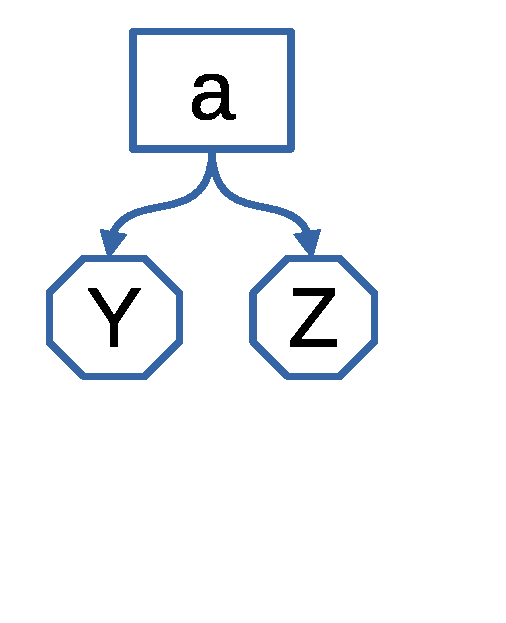
\includegraphics[scale=0.4]{term3.eps} &
    \textbf{\Huge $\Rightarrow$} &
    \pause
    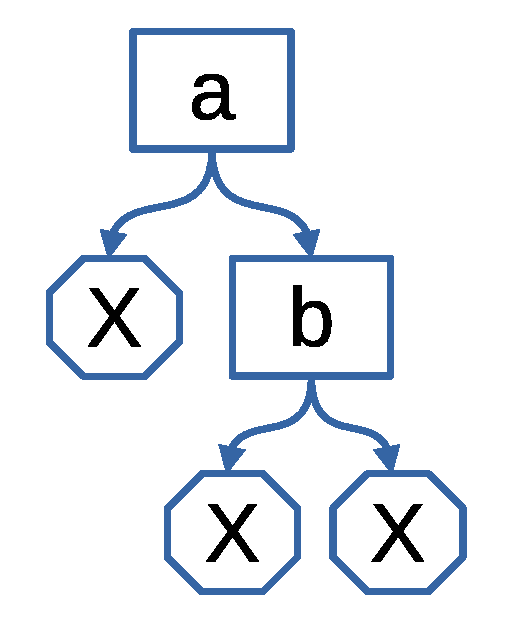
\includegraphics[scale=0.4]{term4.eps}
    \end{tabular}
    \end{frame}

    \begin{frame}
        \frametitle{Унификация: пример 4}
    \begin{tabular}{m{25mm}cm{25mm}cm{25mm}}
    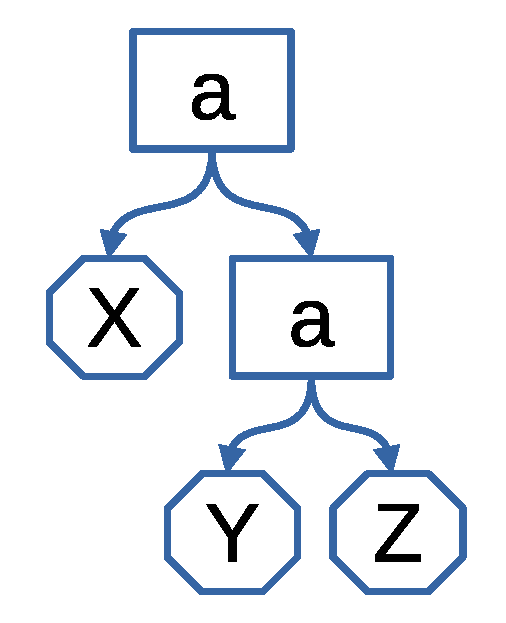
\includegraphics[scale=0.4]{term5.eps} &
    \textbf{\Huge $\equiv$} &
     $\!\!\!\!\!\!$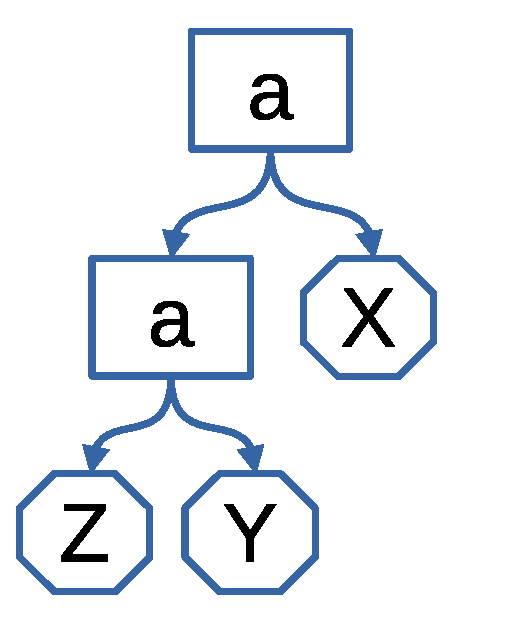
\includegraphics[scale=0.4]{term6.eps} &
    \textbf{\Huge $\Rightarrow$} &
    \pause
    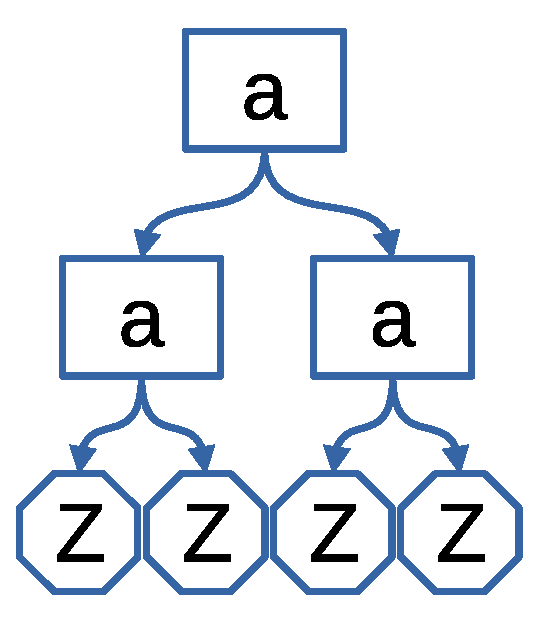
\includegraphics[scale=0.4]{term7.eps}
    \end{tabular}
    \end{frame}

    \begin{frame}
        \frametitle{Унификация: Occurs Check}
    {\Large
    \[
    X \equiv f(X)
    \]}
    \pause
    \begin{itemize}
        \item Некорректно в терминах логики первого порядка
        \begin{itemize}
            \item Результат такой унификации --- $fail$
            \item Детекция вложенности термов замедляет алгоритм унификации
            \item Не детектируется в большинстве реализаций Пролога
        \end{itemize}
        \pause
        \vspace{2mm}
        \item Конечное представление бесконечного терма
        \begin{itemize}
            \item Вероятно, существуют задачи, где такое описание может быть полезным
        \end{itemize}
    \end{itemize}
    \end{frame}

    \begin{frame}[fragile]
        \frametitle{Неполный поиск}
        \begin{minted}{prolog}
:- use_rendering(svgtree).

member(X, leaf(X)).
member(X, node(L, _)) :- member(X, L).
member(X, node(_, R)) :- member(X, R).
        \end{minted}
    \vspace{5mm}
    \begin{itemize}
        \item Проверка наличия значения в листьях дерева
        \pause
        \vspace{2mm}
        \item А если попробовать синтезировать все деревья, содержащие заданное значение в листьях?
    \end{itemize}
    \end{frame}

    \begin{frame}
        \frametitle{Внелогические операторы}
    \begin{itemize}
        \item Оператор отсечения (\mintinline{prolog}{!})
        \begin{itemize}
            \item Запрещает поиск других решений, если одно решение найдено
            \item Позволяет управлять поиском
            \item Недекларативен
        \end{itemize}
        \vspace{2mm}
        \item \mintinline{prolog}{assert} и \mintinline{prolog}{retract}
        \begin{itemize}
            \item Операции динамического добавления и удаления фактов и правил из базы знаний
            \item Позволяют писать мета-программы, изменяющие сами себя в процессе исполнения
        \end{itemize}
        \vspace{2mm}
        \item Negation as Failure
        \vspace{2mm}
        \item И многие другие
    \end{itemize}
    \end{frame}

\end{document}